\chapter{Case study: Social Distancing Students dataset} \label{sec:case_study}
The Social Distancing Students dataset explores dutch public sentiment on governmental COVID-19 measures on Twitter based on data between February to September 2020 \cite{wangPublicSentimentGovernmental2020}.
Public sentiment is an important measure to consider before implementing certain measures or policies as it may influence compliance or cause protests.

The dataset consists of a tweet network encapsulating tweet, retweet, quote, and mention relations and a follower network modeling dynamics of the Twitter social network platform.
The network is constructed by gathering tweets matching a predefined set of keywords related to the COVID-19 crisis.
The follower network is constructed central to the users related to the tweets.
Following the work in the original paper, the dataset contains sentiment analysis labels indicating whether a tweet is in support or rejection of contemporary social distancing policies.

For this case study we have trained the $MGTCOM$ model on the dataset using the same parameters as described in the evaluation (\cref{sec:exp_setup}).
In the following steps, we use the dataset as well as training results to explore the patterns found in the data.
Additionally, we attempt to explain the learned features and communities based on the patterns seen in the data they capture.

\begin{figure}[ht!]
\centering
\subfigure[]{
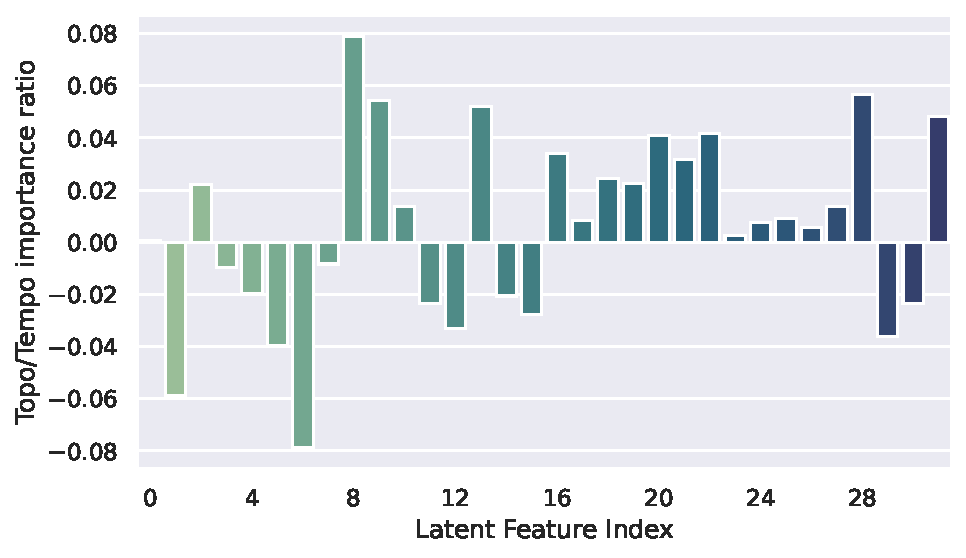
\includegraphics[width=0.47\textwidth]{resources/figs/case_study/02_att_topo_v_tempo.pdf}
}\quad
\subfigure[]{
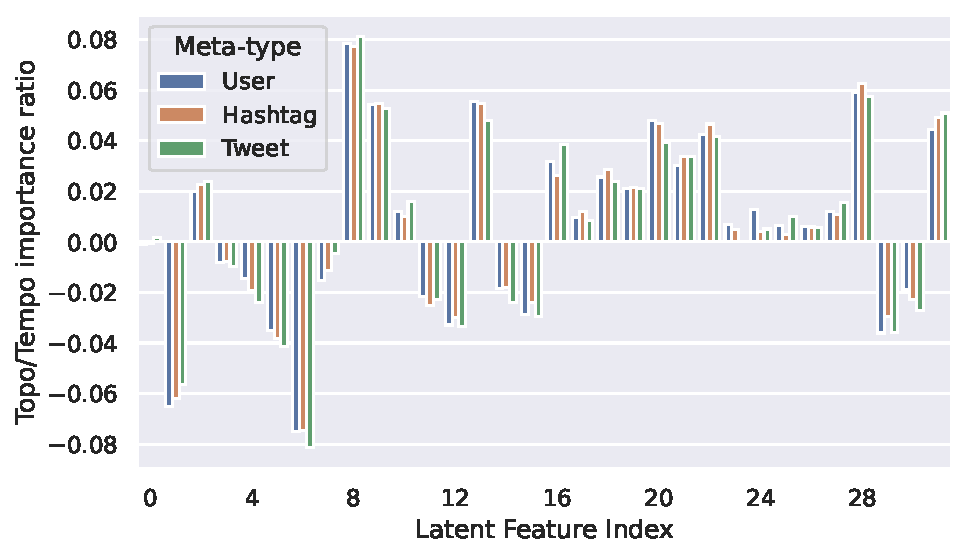
\includegraphics[width=0.47\textwidth]{resources/figs/case_study/03_att_topo_v_tempo_type.pdf}
}\quad
\caption{
    Given a latent feature vector ($d = 32$), for each feature, we plot attention averaged over the whole dataset.
    A positive value means the feature is more important for topological tasks, while a negative value means it is more important for temporal tasks.
    In plot (b) we similarly visualize the attention averaged over data points while grouped by node type.
}
\label{fig:cs_att_ratio}
\end{figure}

In the first step of our analysis, we focus on the relative importance of various embeddings features given their task-specific attention weight.
In \cref{fig:cs_att_ratio} we plot the attention ratio, which is computed as the mean difference between the topological and temporal feature-wise attention ($ATT^{\mathcal{E}} - ATT^{\mathcal{T}}$).
Since, the attention is computed per node, in figure (b) we plot the attention ratio grouped by node type.
While on the feature level a clear distinction is seen where features are more important for either task, we can see that attention between different types doesn't deviate much from the mean.
This is not unexpected as the attention is not parameterized by meta-topology, as it is rather implicitly encoded in the primary embedding vector.

In \cref{fig:cs_tempo_feat_hist} we visualize a temporal histogram for top nodes given individual features that have a higher average temporal attention.
Because our distance measure is based on inner-product, the selection of top nodes works by simply sorting node embeddings by the selected feature in descending order.
In almost all the subplots we see pronounced peaks at certain timestamps indicating that the latent features capture certain temporal patterns within the data.
Since many features capture the peaks during mid-October it is fair to assume that those tweets have certain distinct underlying properties. 
As a baseline, we plot the general tweet distribution over time in \cref{fig:cs_ts_dist} to compare the peaks in feature histograms against.

\begin{figure}[!ht]
\centering
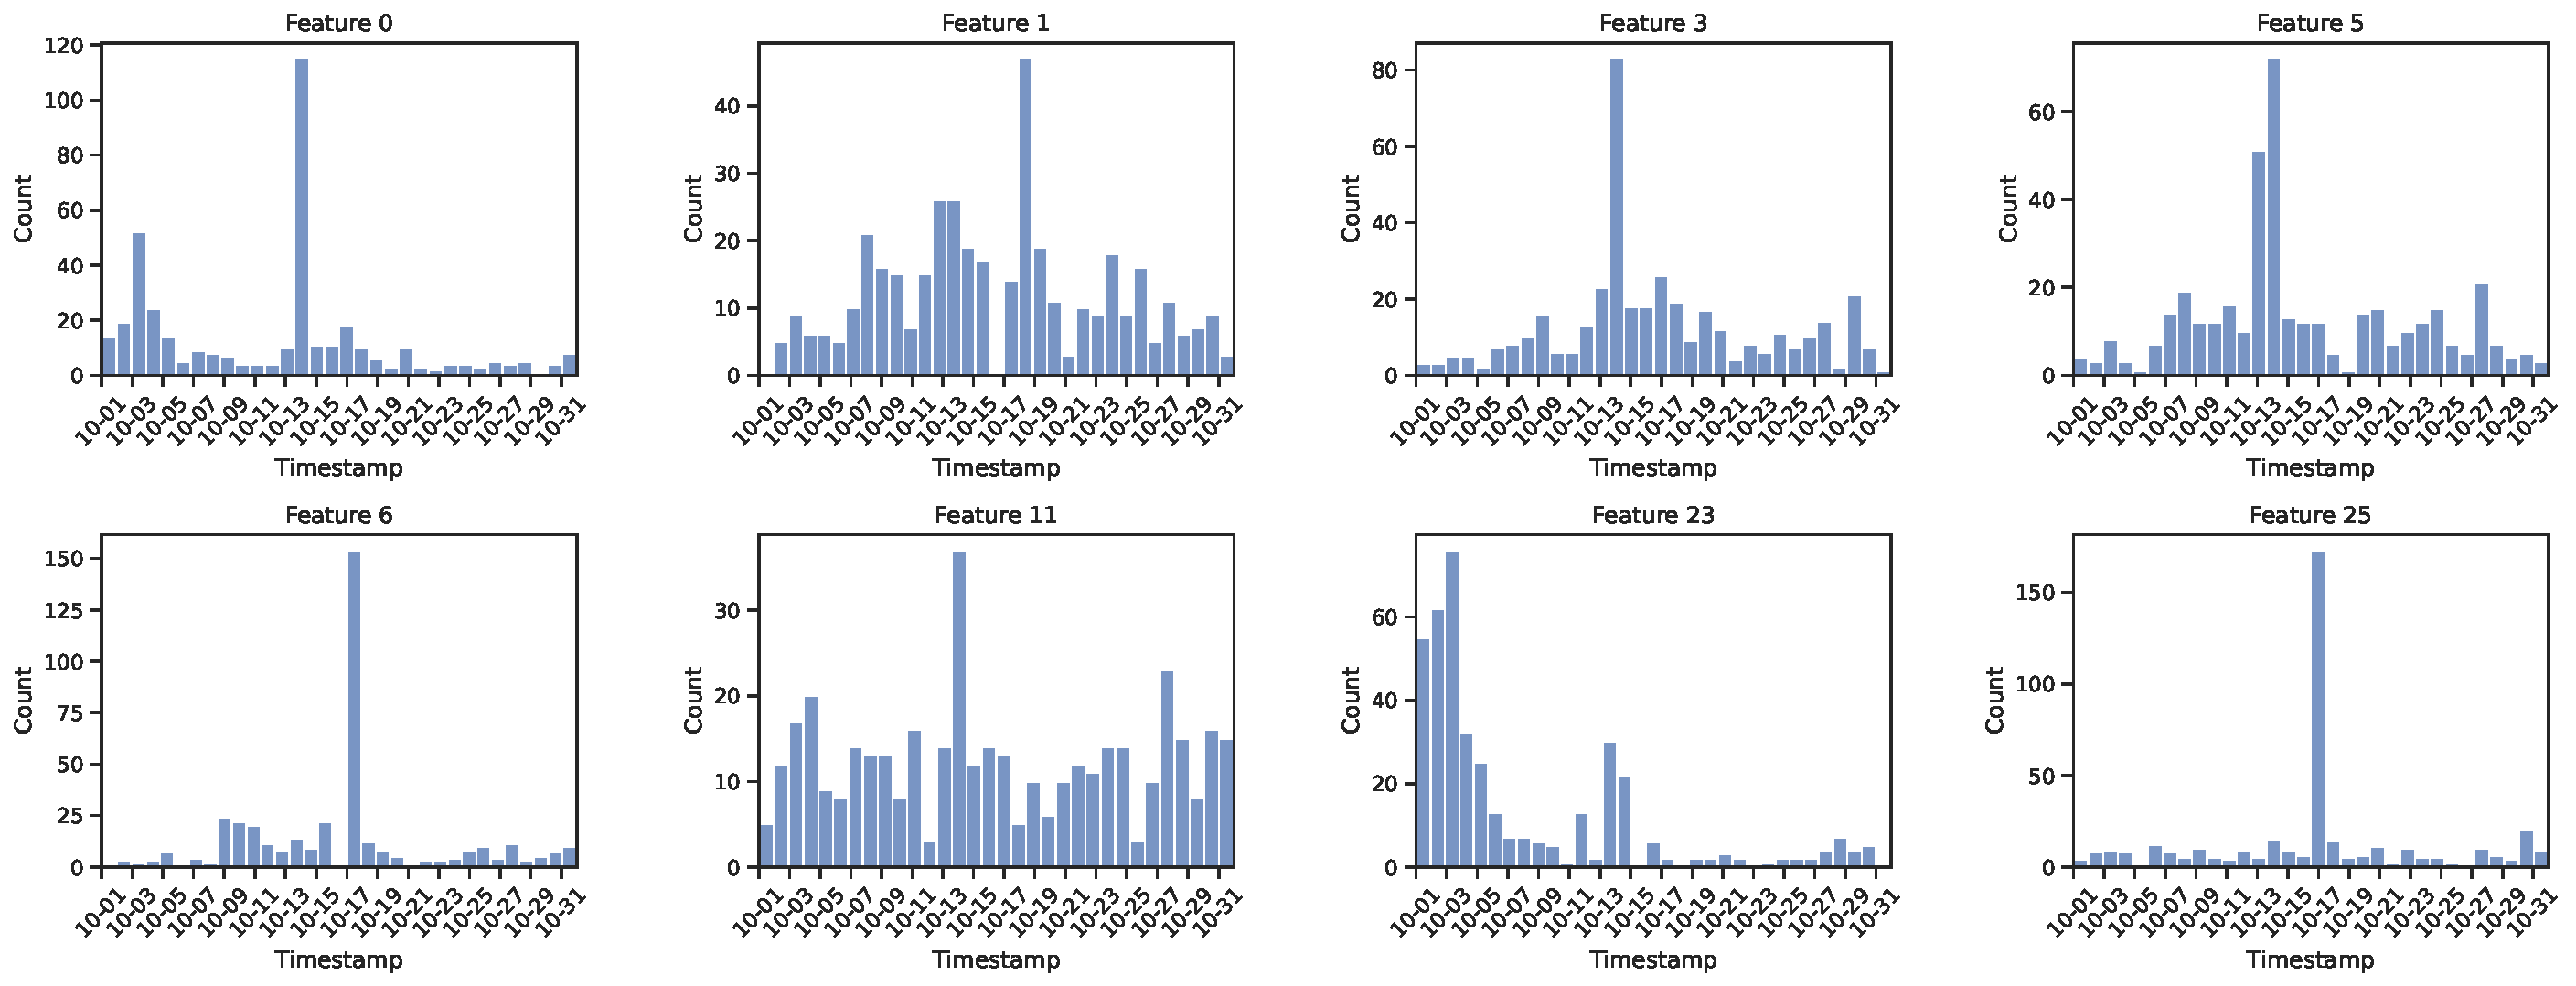
\includegraphics[width=\columnwidth]{resources/figs/case_study/05_att_tempo_hist.pdf}
\caption{
    Distribution of top 200 tweets over time ranked by latent embedding feature which is correlated with high temporal attention.
    The dates on the x-axis are formatted as month-date excluding the year 2021.
}
\label{fig:cs_tempo_feat_hist}
\end{figure}

\begin{figure}[!ht]
\centering
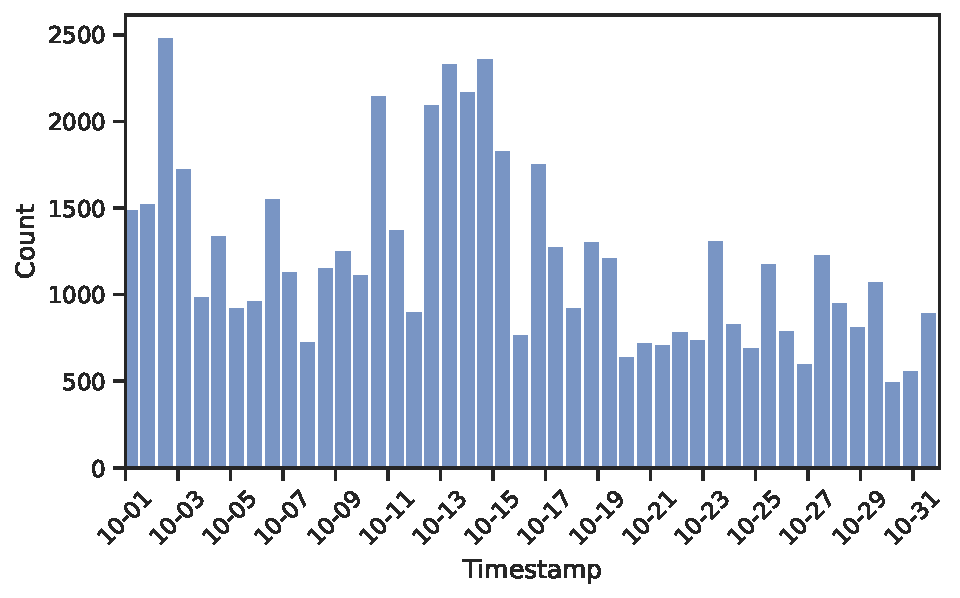
\includegraphics[width=0.5\columnwidth]{resources/figs/case_study/01_timestamp_dist.pdf}
\caption{
    Tweet distribution over time in Social Distancing Students dataset.
}
\label{fig:cs_ts_dist}
\end{figure}

To further study the effectiveness of attended features we plot most common words occurring in top tweets given the attended features in \cref{fig:cs_feat_cloud}.
In these word clouds, we see more explanations for the patterns seen in the temporal histograms.
For latent feature 11 we see the main keywords consisting of "nk", "amsterdam", and "voetbal" referring to contemporary dutch soccer national championship games on 3, 16, 19, 24, and 30th of October.
All the games were played by "Ajax" club based in the city Amsterdam and the dates correspond to the peaks in the histogram.
Similarly, feature 5 contains keywords "dierendag" and "bioindustrie" corresponding to national animal day on 3rd of October and related tweets raising awareness to the bioindustry.
Features 0 and 5 seem to contain more general words referring to trending hashtags ("\#scholenveilig" translated school safe) in anticipation to the press conference from the Dutch parliament on 18th of October.

\begin{figure}[!ht]
\centering
\subfigure[]{
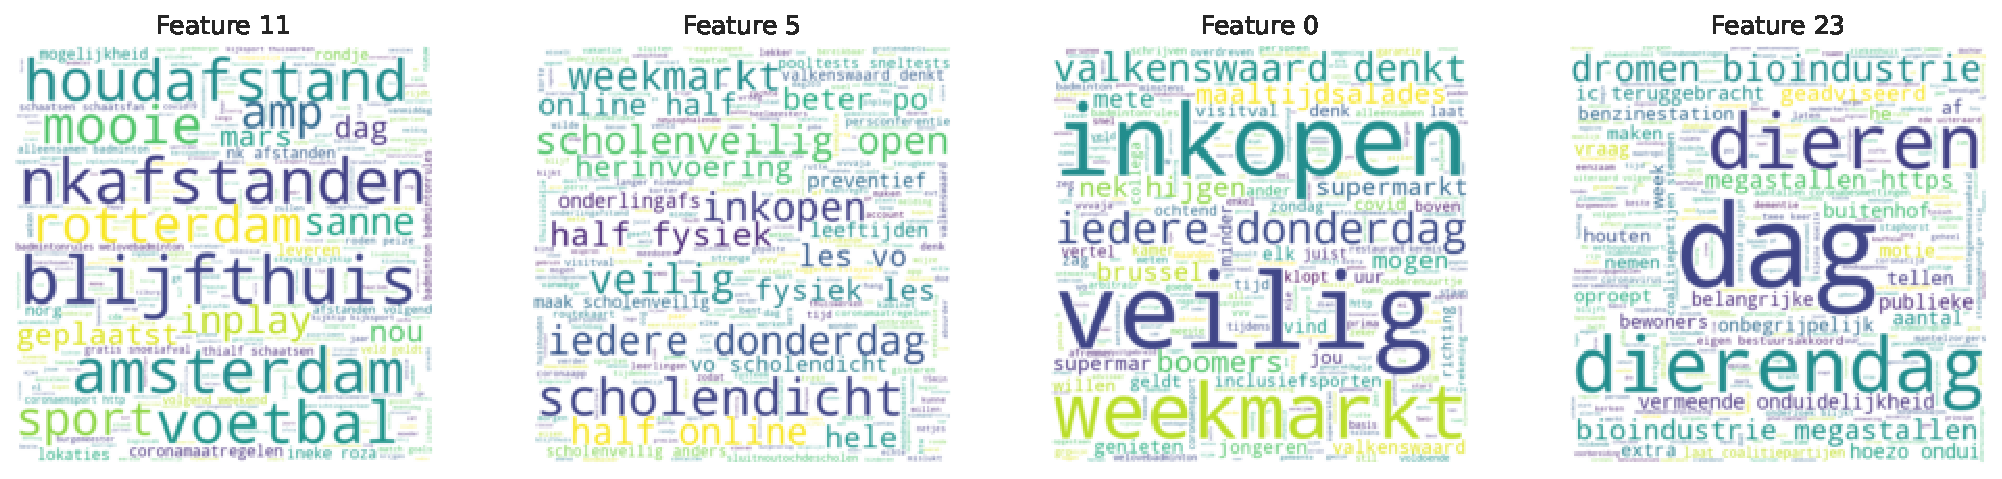
\includegraphics[width=\textwidth]{resources/figs/case_study/06_att_tempo_cloud.pdf}
}\quad
\subfigure[]{
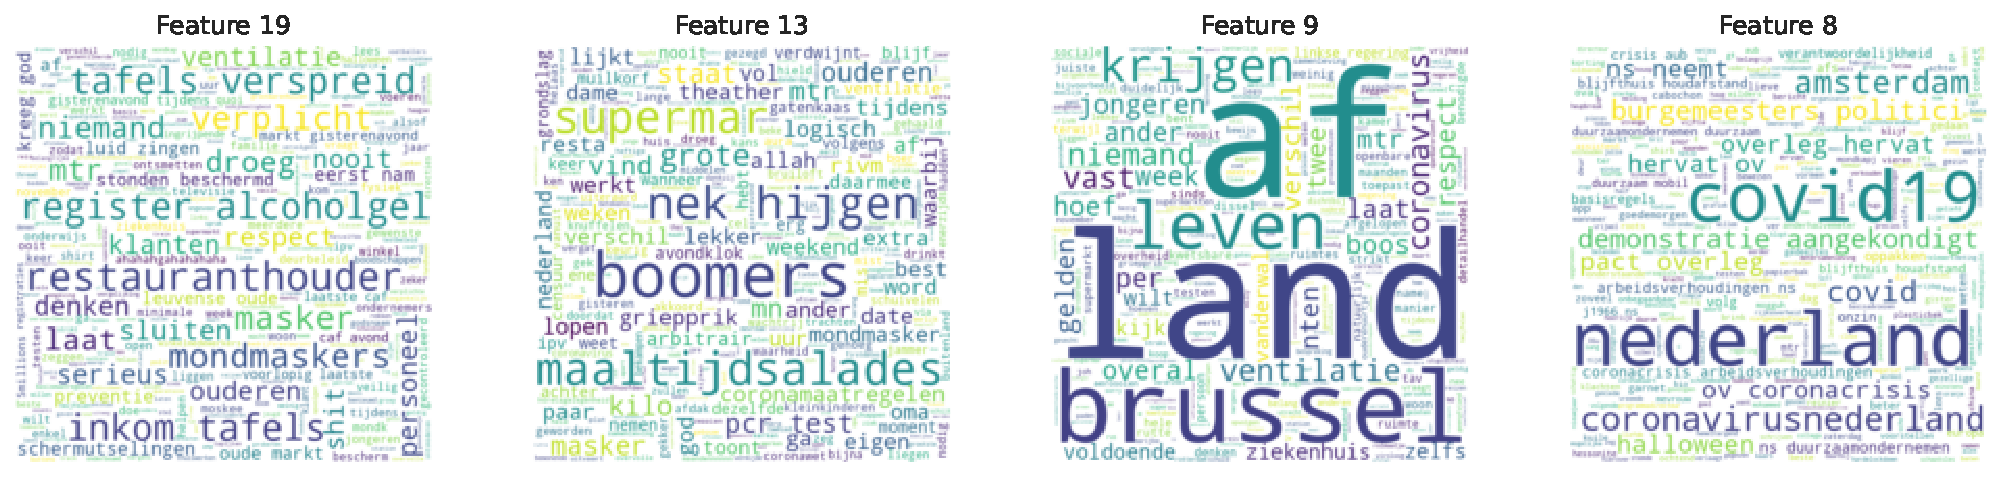
\includegraphics[width=\textwidth]{resources/figs/case_study/04_att_topo_cloud.pdf}
}\quad
\caption{
    Most common words occurring in the top 200 tweets given (a) temporally correlated latent features, (b) topologically correlated latent features.
}
\label{fig:cs_feat_cloud}
\end{figure}

While topological information is gathered from neighboring nodes, it can still tell us about trends on Twitter regarding hashtags and mentions.
In \cref{fig:cs_feat_cloud} (b) we similarly plot keywords for the most valuable/attended topological features.
There we see in features 19 and 13 keywords regarding measures for restaurants and grocery stores respectively.
Feature 8 mainly contains travel keywords such as "ov" and "ns" referring to travel providers, while feature 9 is more focussed on foreign affairs citing city "Brussels" and country ("land").

Next, we are interested in the predictive capability of the embeddings on the sentiment labels provided in the dataset.
In \cref{fig:cs_sentiment_embedding} we see a plot of the two most correlated latent embedding features colored by the sentiment label.
As the predictive accuracy on the label is 81\% and does not greatly exceed 79\% most frequent label baseline, it is fair to assume that the embeddings do not really capture the sentiment of the tweet contents. 

\begin{figure}[]
\centering
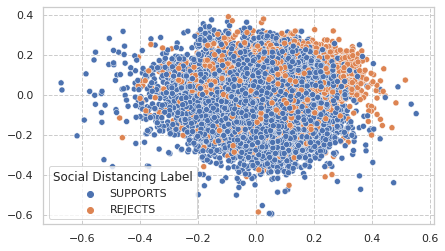
\includegraphics[width=0.5\columnwidth]{resources/figs/case_study/08_embedding_sentiment_best.png}
\caption{
    Visualization of two latent embedding features most correlated with social distancing sentiment.
    Each of the data points is colored corresponding to the sentiment label indicating that the content of the tweet is either for or against a certain measure.
}
\label{fig:cs_sentiment_embedding}
\end{figure}

\begin{figure}[]
\centering
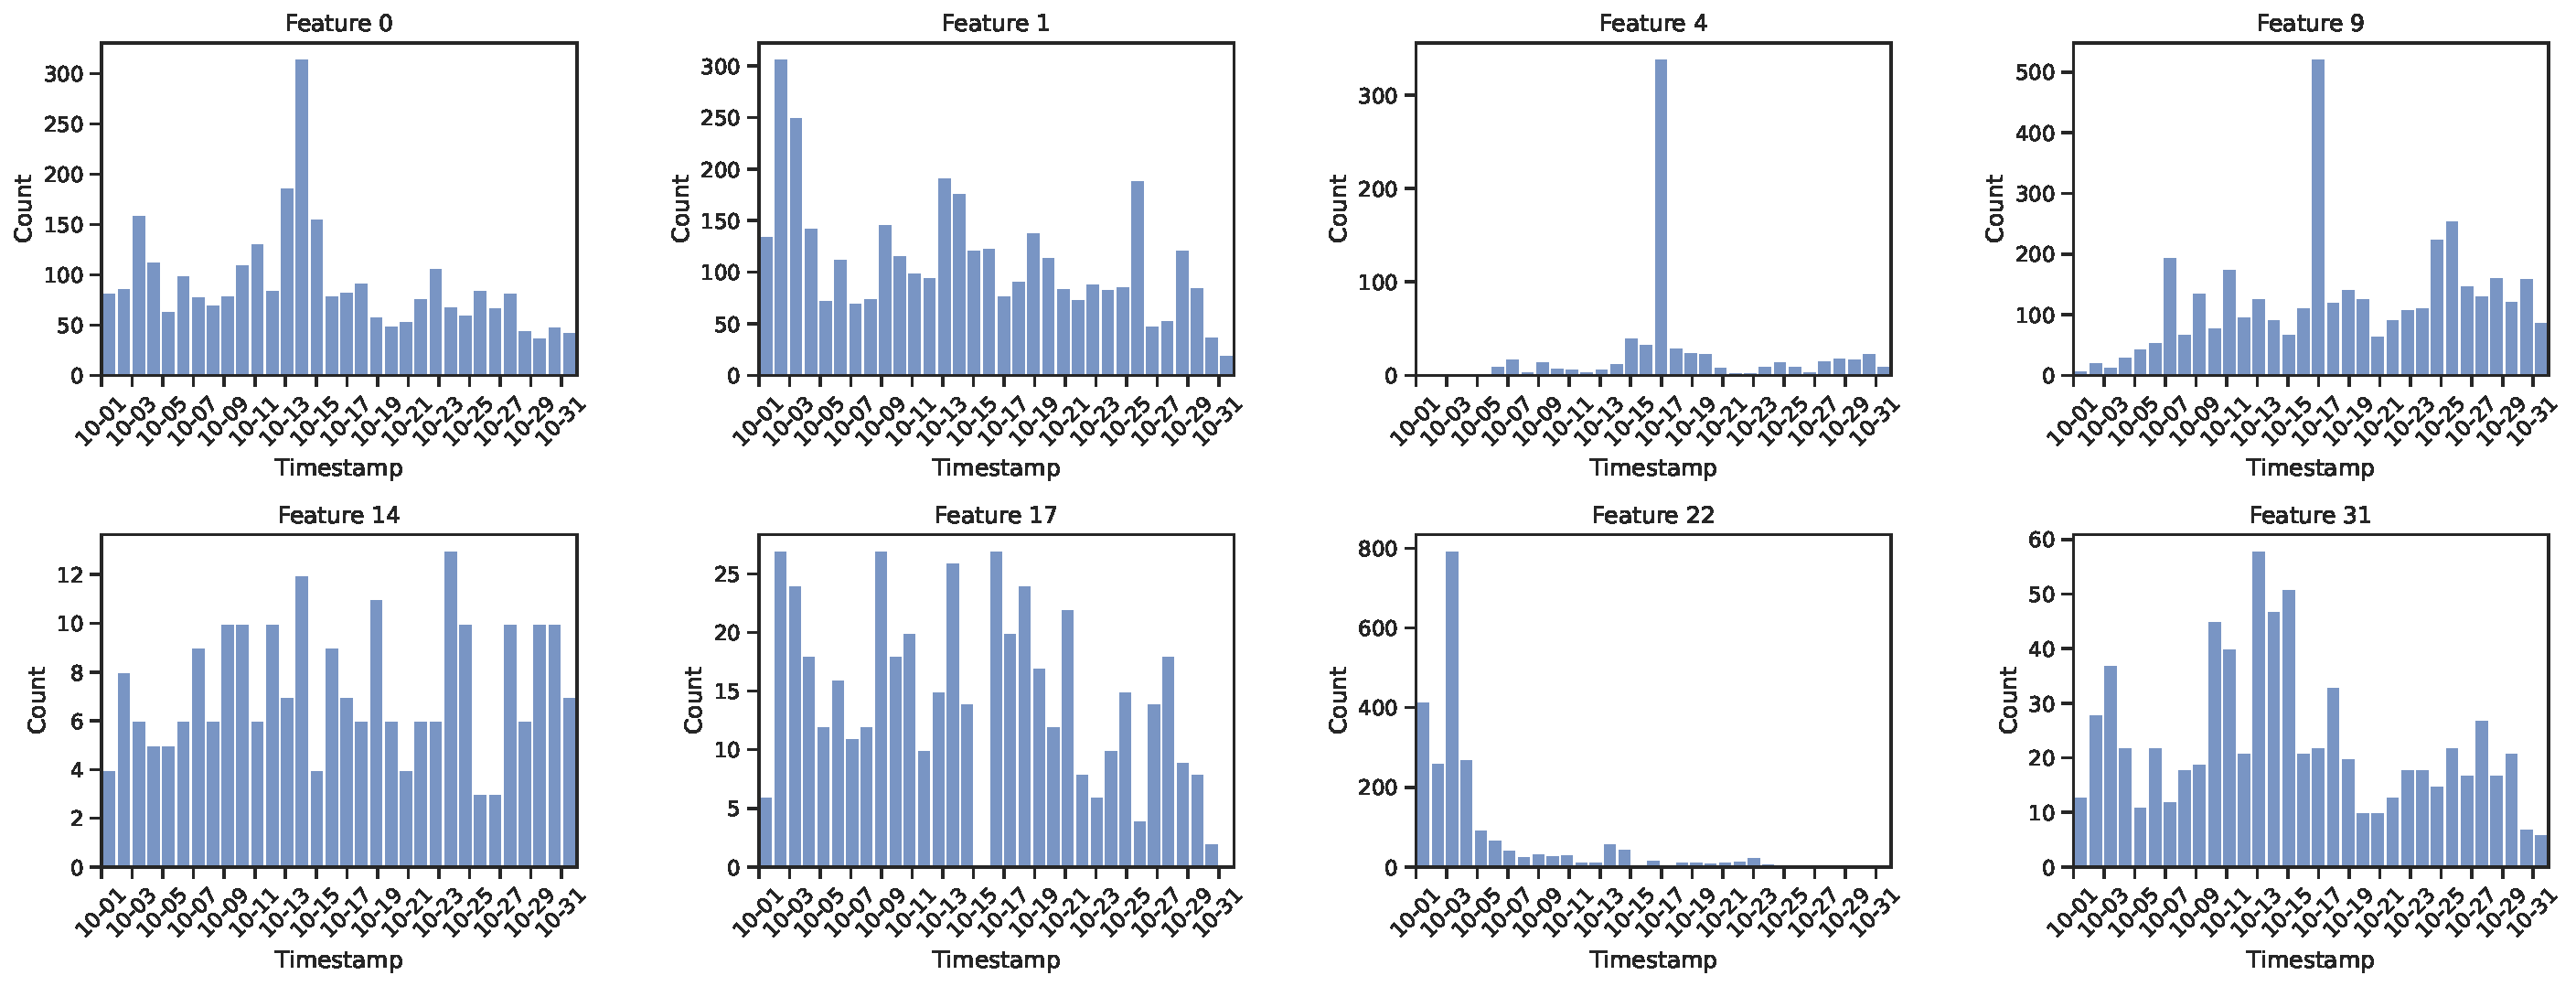
\includegraphics[width=\columnwidth]{resources/figs/case_study/09_cluster_timestamp_dist.pdf}
\caption{
    Distribution of tweets given their respective communities over time. 
}
\label{fig:cs_cluster_time_hist}
\end{figure}

Finally, we analyze the patterns captured by the found communities. 
In \cref{fig:cs_cluster_time_hist} we visualize temporal distribution of Tweets given their corresponding communities.
Contrary to temporal patterns, we see that the communities are mixed in their temporal correlation. 
For example, cluster 14 has a distinct timestamp while cluster 4 is clearly centered around the 17th of October. 

To get more insight into the nature of found communities we plot node type distributions for the found communities in \cref{fig:cs_cluster_type_dist} (a) alongside the node type distribution of the whole dataset.
Aside from mixed-type communities we also see pure communities emerge capturing only follower network data or the tweet data.
Surprisingly, while hashtags make up a small portion of the dataset, we see multiple communities containing a non-trivial fraction of hashtags.

\begin{figure}[!ht]
\centering
\subfigure[]{
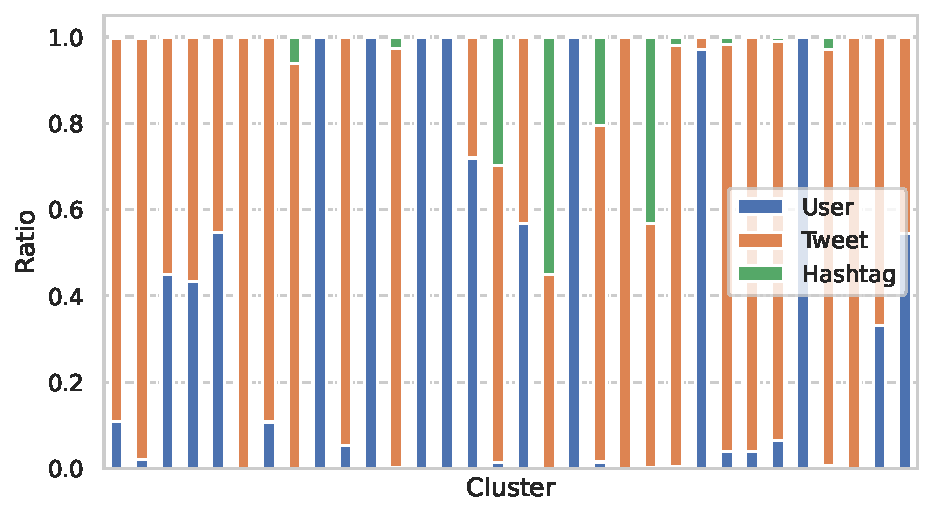
\includegraphics[width=0.5\textwidth]{resources/figs/case_study/10_cluster_type_dist.pdf}
}\quad
\subfigure[]{
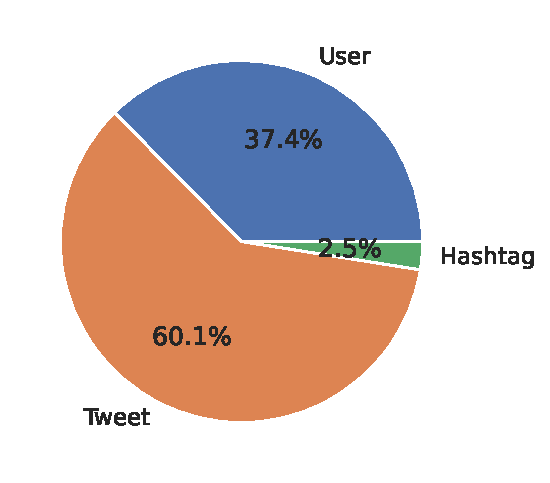
\includegraphics[width=0.3\textwidth]{resources/figs/case_study/11_global_type_dist.pdf}
}\quad
\caption{
    Distribution of node types ("User", "Tweet", "Hashtag") over the (a) found communities, (b) the full dataset.
}
\label{fig:cs_cluster_type_dist}
\end{figure}

Similarly, various patterns the communities capture can be analyzed using the word clouds in \cref{fig:cs_cluster_cloud}.
There we see more pronounced patterns concerning grocery store policies (feature 1), the overfull hospitals (feature 5) and disease transmission (feature 6).

We conclude this section by noting that the found communities capture patterns by combining similar nodes in terms of content, time events and connections together which is very useful for explorative analysis. 
This approach is unsuitable for predicting complex patterns such as support for specific policies as it is not encapsulated in the objective function.
A more suitable way to capture such feature would use representation vectors for all sentence tokens, instead of  the full text average we use currently.
We leave exploration of ways to incorporate such feature extraction into graph embedding pipeline as future work. 

\begin{figure}[!ht]
\centering
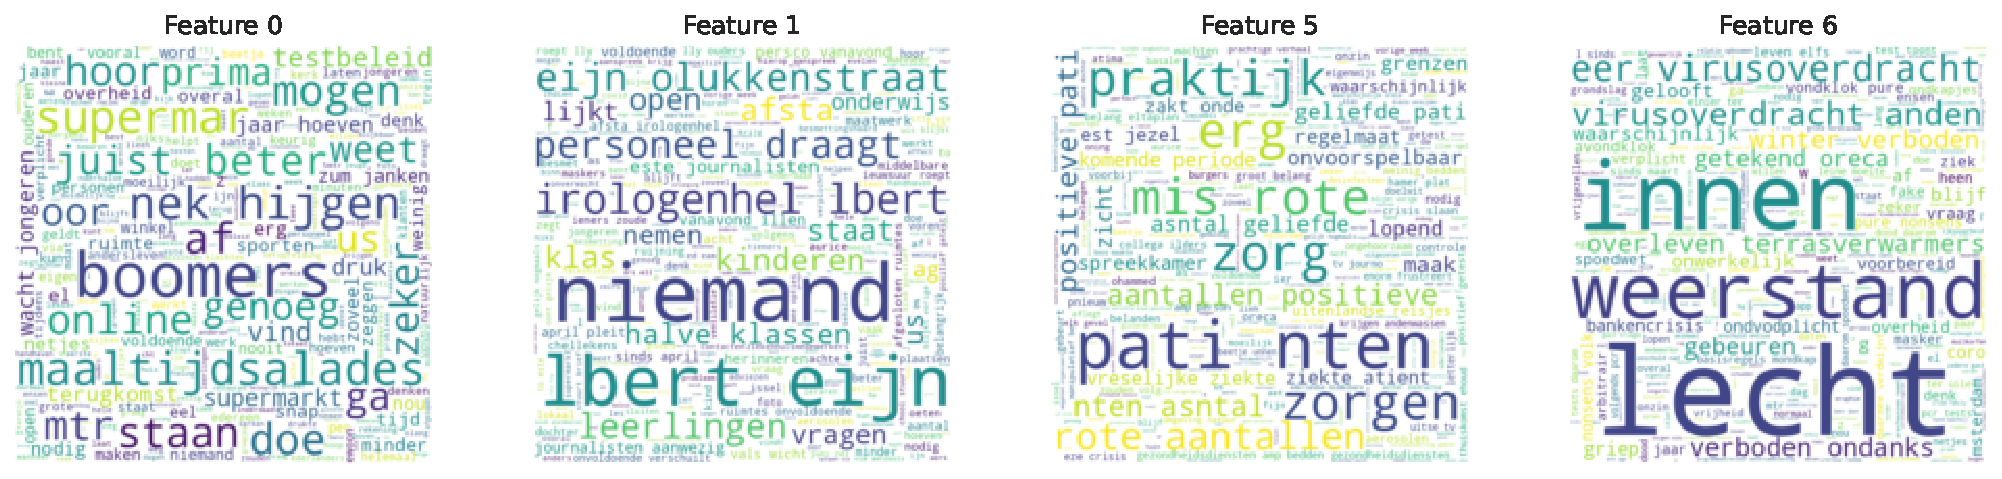
\includegraphics[width=\columnwidth]{resources/figs/case_study/12_cluster_cloud.pdf}
\caption{
    Most common words occurring in various communities.
}
\label{fig:cs_cluster_cloud}
\end{figure}